\documentclass[12pt]{article}
\usepackage[utf8]{inputenc}
\usepackage{amsmath}
\usepackage{amssymb}
\usepackage{mathtools}
\usepackage{amsfonts}
\usepackage{lastpage}
\usepackage{tikz}
\usepackage{pdfpages}
\usepackage{gauss}
\usepackage{fancyvrb}
\usepackage{fancyhdr}
\usepackage{graphicx}
\usepackage{boxproof}
\usepackage{a4wide}
\usepackage{daymonthyear}

\def\meta#1{\mbox{$\langle\hbox{#1}\rangle$}}
\def\macrowitharg#1#2{{\tt\string#1\bra\meta{#2}\ket}}

{\escapechar-1 \xdef\bra{\string\{}\xdef\ket{\string\}}}

\def\intro#1{{#1}{\cal I}}
\def\elim#1{{#1}{\cal E}}

\showboxbreadth 999
\showboxdepth 999
\tracingoutput 1


\let\imp\to
\def\elim#1{{{#1}{\cal E}}}
\def\intro#1{{{#1}{\cal I}}}
\def\lt{<}
\def\eqdef{=}
\def\eps{\mathrel{\epsilon}}
\def\biimplies{\leftrightarrow}
\def\flt#1{\mathrel{{#1}^\flat}}
\def\setof#1{{\left\{{#1}\right\}}}
\let\implies\to
\def\KK{{\mathsf K}}
\let\squashmuskip\relax
\pagestyle{fancy}
\fancyfoot[C]{\footnotesize Page \thepage\ of 21}
\DeclareGraphicsExtensions{.pdf,.png,.jpg}
\title{Elementær Talteori}
\author{Nikolaj Dybdahl Rathcke}
\chead{Nikolaj Dybdahl Rathcke (rfq695)}

\begin{document}
\section*{Logic in Computer Science - Assignment 2}
\subsection*{Exercise 1.2}
\subsubsection*{1r}
We want to prove the validity of the sequent $p\imp q\land r\vdash (p\imp q)\land (p\imp r)$.\\
\begin{proofbox}
   \: p\imp q\land r 	 \=\mbox{premise}\\
   \[
      \: p		  \=\mbox{assumption}\\
      \: q \land r \= \to E(2,1) \\
      \: q \= \land E_1(3)
   \]
   \: p\to q \= I(2-4)
   \[
      \: p		  \=\mbox{assumption}\\
      \: q \land r \= \to E(6,1) \\
      \: r \= \land E_2(7)
   \]
   \: p\to r \= I(6-8) \\
   \: (p\imp q)\land (p\imp r) \= \land I(5,9) \\
\end{proofbox}

\subsubsection*{1s}
We want to prove the validity of the sequent $(p\to q)\land (p\to r)\vdash p\to q\land r$.\\
\begin{proofbox}
   \: (p\to q)\land (p\to r) 	 \=\mbox{premise}\\
   \: p\to q	  \= \land E_1(1)\\
   \: p\to r \= \land E_2(1)
     \[
       \: p		  \=\mbox{assumption}\\
       \: q \= \to E(4,2) \\
       \: r \= \to E(4,3) \\
       \: q\land r \= \land I(5,6)
     \]
   \: p\to q\land r \= \to I(4-7)
\end{proofbox}

\subsubsection*{3q}
We want to prove the validity of the sequent $\vdash (p\to q)\lor (q\to r)$.\\
\begin{proofbox}
     \: q \lor \neg q \= LEM \\
     \[
       \: q		  \=\mbox{assumption}
       \[
         \: p  \=\mbox{assumption} \\
         \: q \= (2)         
       \]
       \: p\to q \= \to I(3-4) \\
       \: (p\to q)\lor (q\to r) \= \lor I_1(5)
     \]
     \[
       \: \neg q		  \=\mbox{assumption}\\
       \[
         \: q \=\mbox{assumption}\\
         \: \bot \= \neg E(8,7) \\
         \: r \= \bot (9)
       \]
       \: q\to r \= \to I(8-10) \\
       \: (p\to q)\lor (q\to r) \= \lor I_2(11)
     \]
     \: (p\to q)\lor (q\to r) \= \lor E(1,2-6,7-12)
\end{proofbox}

\subsubsection*{3u}
We want to prove the validity of the sequent $(s\to p)\lor (t\to q)\vdash (s\to q)\lor (t\to p)$.\\
The proof can be seen on the next page.
\newpage
\begin{proofbox}
     \: (s\to p)\lor (t\to q) \=\mbox{premise}
     \[
       \: s\to p \= \mbox{assumption} \\
       \: s\lor\neg s \= LEM \\
       \[
         \: s \= \mbox{assumption}
         \[
           \: t \= \mbox{assumption} \\
           \: p \= \to E(4,2)
         \]
         \: t\to p \= \to I(5-6) \\
         \: (s\to q)\lor (t\to p) \= \lor I_2(7)
       \]
       \[
         \: \neg s \= \mbox{assumption}
         \[
           \: s \= \mbox{assumption} \\
           \: \bot \= \neg E(10,9) \\
           \: q \= \bot E(11)
         \]
         \: s\to q \= \to I(10-12) \\
         \: (s\to q)\lor (t\to p) \= \lor I_1(13)
       \]
       \: (s\to q)\lor (t\to p) \= \lor E(3,4-8,9-14)
     \]
     \[
       \: t\to q \= \mbox{assumption} \\
       \: t\lor\neg t \= LEM \\
       \[
         \: t \= \mbox{assumption}
         \[
           \: s \= \mbox{assumption} \\
           \: q \= \to E(18,16)
         \]
         \: s\to q \= \to I(19-20) \\
         \: (s\to q)\lor (t\to p) \= \lor I_1(21)
       \]
       \[
         \: \neg t \= \mbox{assumption}
         \[
           \: t \= \mbox{assumption} \\
           \: \bot \= \neg E(24,23) \\
           \: p \= \bot E(25)
         \]
         \: t\to p \= \to I(24-26) \\
         \: (s\to q)\lor (t\to p) \= \lor I_2(27)
       \]
       \: (s\to q)\lor (t\to p) \= \lor E(17,18-22,23-28)
     \]
     \: (s\to q)\lor (t\to p) \= \lor E(1,2-15,16-29)
\end{proofbox}

\subsection*{Exercise 1.4}
\subsubsection*{17a}
We want to show that $\models\phi$ holds for the $\phi$ in $(p\imp q)\lor (q\imp r)$. \\
We construct a truth table\\
\begin{center}
\begin{tabular}{|c|c|c||c|c||c|}
\hline 
$p$ & $q$ & $r$ & $p\to q$ & $q\to r$ & $(p\imp q)\lor (q\imp r)$ \\ 
\hline 
T & T & T & T & T & T \\ 
\hline 
T & T & F & T & F & T \\ 
\hline 
T & F & T & F & T & T \\ 
\hline
F & T & T & T & T & T \\ 
\hline  
T & F & F & F & T & T \\ 
\hline 
F & F & T & T & T & T \\ 
\hline 
F & T & F & T & F & T \\ 
\hline 
F & F & F & T & T & T\\ 
\hline 
\end{tabular} 
\end{center}
And we see it is a tautology.

\subsubsection*{17b}
We want to show that $\models\phi$ holds for the $\phi$ in $((q\to (p\lor(q\to p)))\lor \neg(p\to q))\to p$. \\
We construct a truth table\\
\begin{center}
\begin{tabular}{|c|c||c|}
\hline 
$p$ & $q$ & $((q\to (p\lor(q\to p)))\lor \neg(p\to q))\to p$ \\ 
\hline 
T & T & T \\ 
\hline 
T & F & T \\ 
\hline 
F & T & T \\ 
\hline
F & F & F \\ 
\hline
\end{tabular} 
\end{center}
And we see it is not a tautology and it does not hold.

\subsection*{Exercise 1.5}
\subsubsection*{7b}
We want to construct a CNF. First, we want to express the lines that produces false and then negate every atom in this expression, so
\begin{align*}
(\neg p\lor\neg q\lor r)\land(\neg p\lor q\lor\neg r)\land(\neg p\lor q\lor r)\land(p\lor\neg q\lor r)\land(p\lor q\lor r)
\end{align*}
Which is the final result where there are "and" between every line and there is "or" between all atoms.

\subsubsection*{15a}
We want to apply the \texttt{HORN} algorithm to this Horn formula.
$$(p \land q \land w \imp \bot) \land (t \imp \bot) \land (r \imp p) \land (\top \imp r) \land (\top \imp q) \land (u \imp s) \land (\top \imp u)$$
Step one is marking all $\top$.\\
$$(p \land q \land w \imp \bot) \land (t \imp \bot) \land (r \imp p) \land (\underline{\top} \imp r) \land (\underline{\top} \imp q) \land (u \imp s) \land (\underline{\top} \imp u)$$
Step 2 is now marking all right hand side of an implication where the left side has a $\top$. If an expression is marked, all the occurences of the same expression in the formula are also marked. We keep repeating this until we can not do it anymore, so
\begin{align*}
(p \land q \land w \imp \bot) \land (t \imp \bot) \land (r \imp p) \land (\underline{\top} \imp \underline{r}) \land (\underline{\top} \imp \underline{q}) \land (u \imp s) \land (\underline{\top} \imp \underline{u}) \\
(p \land \underline{q} \land w \imp \bot) \land (t \imp \bot) \land (\underline{r} \imp p) \land (\underline{\top} \imp \underline{r}) \land (\underline{\top} \imp \underline{q}) \land (\underline{u} \imp s) \land (\underline{\top} \imp \underline{u}) \\
(p \land \underline{q} \land w \imp \bot) \land (t \imp \bot) \land (\underline{r} \imp \underline{p}) \land (\underline{\top} \imp \underline{r}) \land (\underline{\top} \imp \underline{q}) \land (\underline{u} \imp \underline{s}) \land (\underline{\top} \imp \underline{u}) \\
(\underline{p} \land \underline{q} \land w \imp \bot) \land (t \imp \bot) \land (\underline{r} \imp \underline{p}) \land (\underline{\top} \imp \underline{r}) \land (\underline{\top} \imp \underline{q}) \land (\underline{u} \imp \underline{s}) \land (\underline{\top} \imp \underline{u})
\end{align*}
Since no $\bot$ are marked, step 3 tell us to go to step 4.\\
Step 4 tell us that "The Horn formula is satisfiable".

\subsubsection*{15c}
We want to apply the \texttt{HORN} algorithm to this Horn formula.
$$(p\land q\land s\to p)\land(q\land r\to p)\land(p\land s\to s)$$
Since there are no $\top$, we can not mark anything, so we proceed to step 2.\\
Since nothing is marked, we not mark anything in step 2, so we go to step 3.\\
Since no $\bot$ are marked, we can go to step 4.\\
Step 4 tell us that the Horn formula is satisfiable.

\subsubsection*{15f}
We want to apply the \texttt{HORN} algorithm to this Horn formula.
$$(\top\to q)\land(\top\to s)\land(w\to\bot)\land(p\land q\land s\to\bot)\land(v\to s)\land(\top\to r)\land(r\to p)$$
In step 1, we mark all $\top$ again
$$(\underline{\top}\to q)\land(\underline{\top}\to s)\land(w\to\bot)\land(p\land q\land s\to\bot)\land(v\to s)\land(\underline{\top}\to r)\land(r\to p)$$
Now as completed in step 2, we keep marking expressions until we can not do it anymore.
\begin{align*}
(\underline{\top}\to \underline{q})\land(\underline{\top}\to \underline{s})\land(w\to\bot)\land(p\land q\land s\to\bot)\land(v\to s)\land(\underline{\top}\to \underline{r})\land(r\to p) \\
(\underline{\top}\to \underline{q})\land(\underline{\top}\to \underline{s})\land(w\to\bot)\land(p\land \underline{q}\land \underline{s}\to\bot)\land(v\to \underline{s})\land(\underline{\top}\to \underline{r})\land(\underline{r}\to p) \\
(\underline{\top}\to \underline{q})\land(\underline{\top}\to \underline{s})\land(w\to\bot)\land(p\land \underline{q}\land \underline{s}\to\bot)\land(v\to \underline{s})\land(\underline{\top}\to \underline{r})\land(\underline{r}\to \underline{p}) \\
(\underline{\top}\to \underline{q})\land(\underline{\top}\to \underline{s})\land(w\to\bot)\land(\underline{p}\land \underline{q}\land \underline{s}\to\bot)\land(v\to \underline{s})\land(\underline{\top}\to \underline{r})\land(\underline{r}\to \underline{p}) \\
(\underline{\top}\to \underline{q})\land(\underline{\top}\to \underline{s})\land(w\to\bot)\land(\underline{p}\land \underline{q}\land \underline{s}\to\underline{\bot})\land(v\to \underline{s})\land(\underline{\top}\to \underline{r})\land(\underline{r}\to \underline{p})
\end{align*}
We can no longer repeat step 2, so we proceed to step 3.\\
Since there is one marked $\bot$, step 3 tells us that "The Horn formula is unsatisfiable".

\subsection*{Exercise 1.6}
\subsection*{9a}
We need to show that tests for the tree in [H\& R, page 77] produces contradictory constraints.\\ 
In the following, $X$ is a produced contradictory constraint. \\
\begin{picture}(205,240)
\put(0,0){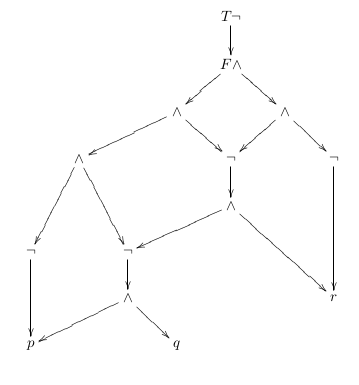
\includegraphics[scale=0.6]{tree.png}}
\put(95,162){a}
\put(157,162){b}
\put(33,134){c}
\put(125,134){d}
\put(185,134){e}
\put(125,107){f}
\put(7,75){g}
\put(65,75){h}
\put(65,50){i}
\put(185,50){j}
\put(7,20){k}
\put(95,20){l}
\end{picture}
\begin{picture}(205,240)
\put(0,0){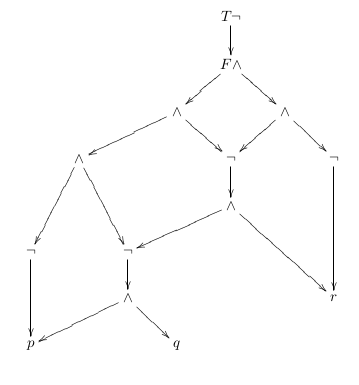
\includegraphics[scale=0.6]{tree.png}}
\put(95,162){T}
\put(157,162){b}
\put(33,134){c}
\put(125,134){d}
\put(185,134){e}
\put(125,107){f}
\put(7,75){g}
\put(65,75){h}
\put(65,50){i}
\put(185,50){j}
\put(7,20){k}
\put(95,20){l}
\end{picture}
\\
On the left side, we have the tree and its nodes labeled by letter to easily refer to them. We are gonna use these labels in both 9a and 9b. We start the test by setting the node $a$ to $T$.\\
\begin{picture}(205,240)
\put(0,0){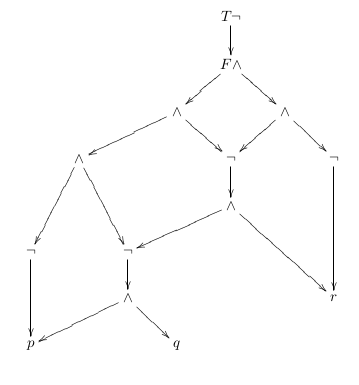
\includegraphics[scale=0.6]{tree.png}}
\put(95,162){T}
\put(157,162){F}
\put(33,134){T}
\put(125,134){T}
\put(185,134){e}
\put(125,107){f}
\put(7,75){g}
\put(65,75){h}
\put(65,50){i}
\put(185,50){j}
\put(7,20){k}
\put(95,20){l}
\end{picture}
\begin{picture}(205,240)
\put(0,0){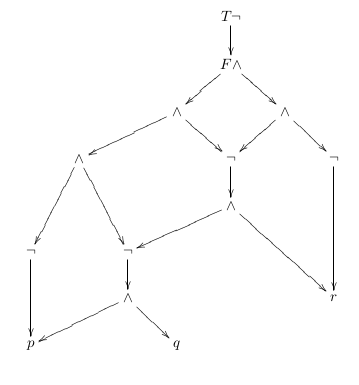
\includegraphics[scale=0.6]{tree.png}}
\put(95,162){T}
\put(157,162){b}
\put(33,134){c}
\put(125,134){d}
\put(185,134){e}
\put(125,107){f}
\put(7,75){g}
\put(65,75){h}
\put(65,50){i}
\put(185,50){j}
\put(7,20){k}
\put(95,20){l}
\end{picture}
\\
Left tree: We see that $a=T$ has forced $b=F$ and for $a$ to be true, this means that both $c$ and $d$ are forced to be true.\\
Right tree: Since $d=T$, this means that node $f$ is forced to be false. Likewise, because $e=F$ this means that node $j$ (or the atom $r$) has to be true.\\
\begin{center}
\begin{picture}(205,240)
\put(0,0){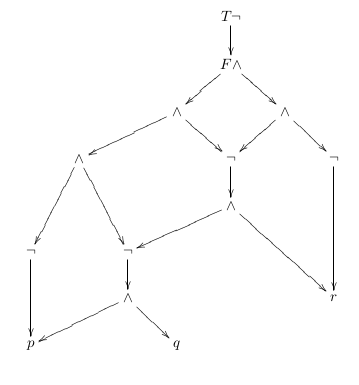
\includegraphics[scale=0.6]{tree.png}}
\put(95,162){T}
\put(157,162){F}
\put(33,134){T}
\put(125,134){T}
\put(185,134){F}
\put(125,107){F}
\put(7,75){T}
\put(65,75){X}
\put(65,50){i}
\put(185,50){T}
\put(7,20){k}
\put(95,20){l}
\end{picture}
\end{center}
Now that node $f$ is false and node $j$ is true, this forces $h=F$. However, we see that node $c$ is true and thus forces $g$ and $h$ to be true. This means we have produced a contradictory constraint.

\subsection*{9b}
Since we saw in (9a) that marking node $a$ to true would result in contradictory constraints, we know this is false. We now try all the possibilities. \\
\begin{picture}(205,240)
\put(0,0){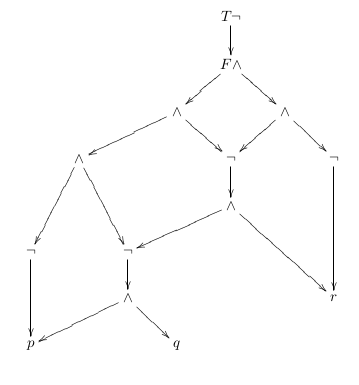
\includegraphics[scale=0.6]{tree.png}}
\put(95,162){F}
\put(157,162){T}
\put(33,134){F}
\put(125,134){T}
\put(185,134){T}
\put(125,107){F}
\put(7,75){g}
\put(65,75){h}
\put(65,50){i}
\put(185,50){F}
\put(7,20){k}
\put(95,20){l}
\end{picture}
\begin{picture}(205,240)
\put(0,0){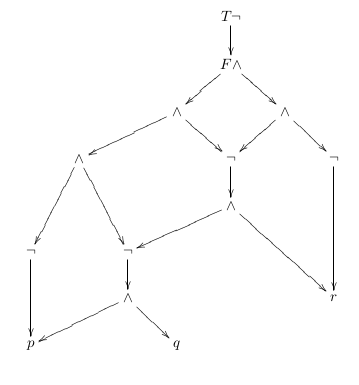
\includegraphics[scale=0.6]{tree.png}}
\put(95,162){T}
\put(157,162){F}
\put(33,134){c}
\put(125,134){d}
\put(185,134){e}
\put(125,107){f}
\put(7,75){g}
\put(65,75){h}
\put(65,50){i}
\put(185,50){j}
\put(7,20){k}
\put(95,20){l}
\end{picture}
\\
In the trees above, we have tried setting node $b$ to $T$ and $F$. We see that we can set no permanent marks and we find no contradictory constraints.\\
\begin{picture}(205,240)
\put(0,0){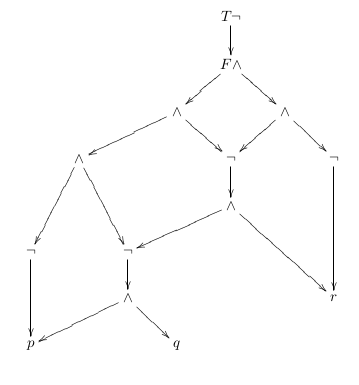
\includegraphics[scale=0.6]{tree.png}}
\put(95,162){F}
\put(157,162){F}
\put(33,134){T}
\put(125,134){F}
\put(185,134){F}
\put(125,107){T}
\put(7,75){T}
\put(65,75){T}
\put(65,50){F}
\put(185,50){T}
\put(7,20){F}
\put(95,20){l}
\end{picture}
\begin{picture}(205,240)
\put(0,0){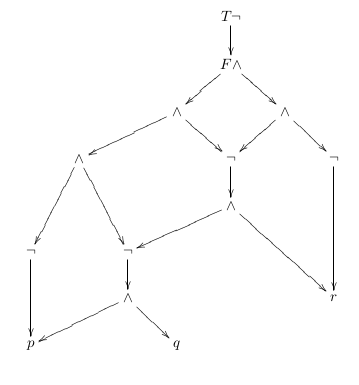
\includegraphics[scale=0.6]{tree.png}}
\put(95,162){F}
\put(157,162){b}
\put(33,134){F}
\put(125,134){d}
\put(185,134){e}
\put(125,107){f}
\put(7,75){g}
\put(65,75){h}
\put(65,50){i}
\put(185,50){j}
\put(7,20){k}
\put(95,20){l}
\end{picture}
\\
In the trees above, we have tried setting node $c$ to $T$ and $F$. We see that we can set no permanent marks and we find no contradictory constraints.\\
\begin{picture}(205,240)
\put(0,0){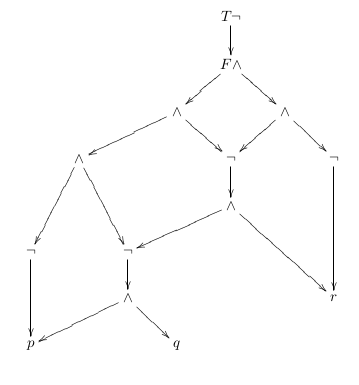
\includegraphics[scale=0.6]{tree.png}}
\put(95,162){F}
\put(157,162){b}
\put(33,134){F}
\put(125,134){T}
\put(185,134){e}
\put(125,107){F}
\put(7,75){g}
\put(65,75){h}
\put(65,50){i}
\put(185,50){j}
\put(7,20){k}
\put(95,20){l}
\end{picture}
\begin{picture}(205,240)
\put(0,0){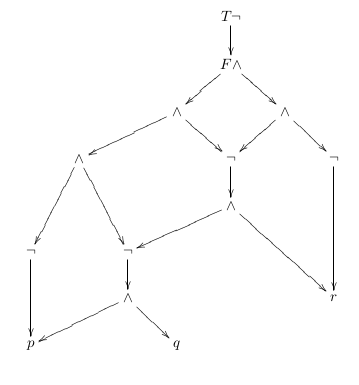
\includegraphics[scale=0.6]{tree.png}}
\put(95,162){F}
\put(157,162){F}
\put(33,134){c}
\put(125,134){F}
\put(185,134){F}
\put(125,107){T}
\put(7,75){g}
\put(65,75){T}
\put(65,50){F}
\put(185,50){T}
\put(7,20){k}
\put(95,20){l}
\end{picture}
\\
In the trees above, we have tried setting node $d$ to $T$ and $F$. We see that we can set no permanent marks and we find no contradictory constraints.\\
\begin{picture}(205,240)
\put(0,0){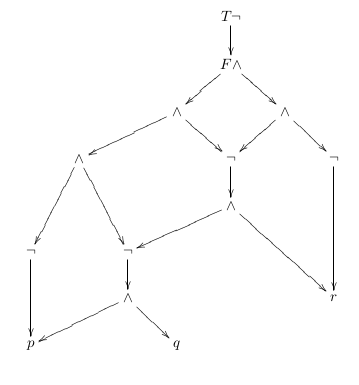
\includegraphics[scale=0.6]{tree.png}}
\put(95,162){F}
\put(157,162){T}
\put(33,134){F}
\put(125,134){T}
\put(185,134){T}
\put(125,107){F}
\put(7,75){g}
\put(65,75){h}
\put(65,50){i}
\put(185,50){F}
\put(7,20){k}
\put(95,20){l}
\end{picture}
\begin{picture}(205,240)
\put(0,0){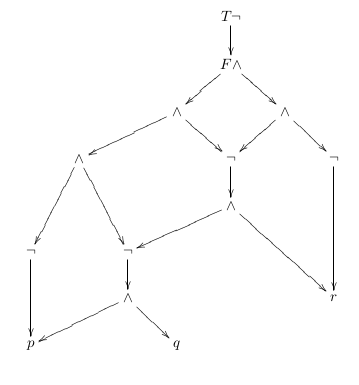
\includegraphics[scale=0.6]{tree.png}}
\put(95,162){F}
\put(157,162){F}
\put(33,134){c}
\put(125,134){d}
\put(185,134){F}
\put(125,107){f}
\put(7,75){g}
\put(65,75){h}
\put(65,50){i}
\put(185,50){T}
\put(7,20){k}
\put(95,20){l}
\end{picture}
\\
In the trees above, we have tried setting node $e$ to $T$ and $F$. We see that we can set no permanent marks and we find no contradictory constraints.\\
\begin{picture}(205,240)
\put(0,0){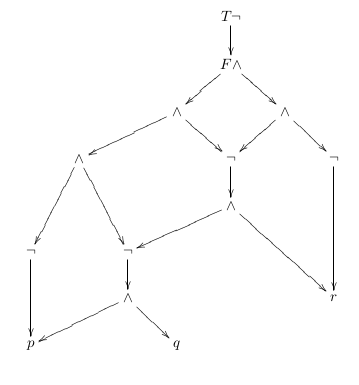
\includegraphics[scale=0.6]{tree.png}}
\put(95,162){F}
\put(157,162){F}
\put(33,134){c}
\put(125,134){F}
\put(185,134){F}
\put(125,107){T}
\put(7,75){g}
\put(65,75){T}
\put(65,50){F}
\put(185,50){T}
\put(7,20){k}
\put(95,20){l}
\end{picture}
\begin{picture}(205,240)
\put(0,0){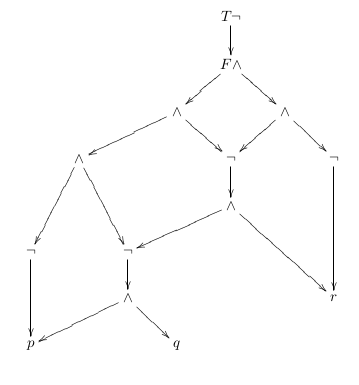
\includegraphics[scale=0.6]{tree.png}}
\put(95,162){F}
\put(157,162){b}
\put(33,134){c}
\put(125,134){T}
\put(185,134){e}
\put(125,107){F}
\put(7,75){g}
\put(65,75){h}
\put(65,50){i}
\put(185,50){j}
\put(7,20){k}
\put(95,20){l}
\end{picture}
\\
In the trees above, we have tried setting node $f$ to $T$ and $F$. We see that we can set no permanent marks and we find no contradictory constraints.\\
\begin{picture}(205,240)
\put(0,0){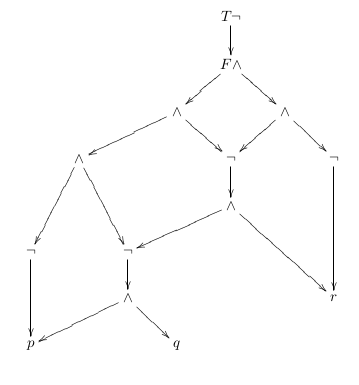
\includegraphics[scale=0.6]{tree.png}}
\put(95,162){F}
\put(157,162){F}
\put(33,134){T}
\put(125,134){F}
\put(185,134){F}
\put(125,107){T}
\put(7,75){T}
\put(65,75){T}
\put(65,50){F}
\put(185,50){T}
\put(7,20){F}
\put(95,20){l}
\end{picture}
\begin{picture}(205,240)
\put(0,0){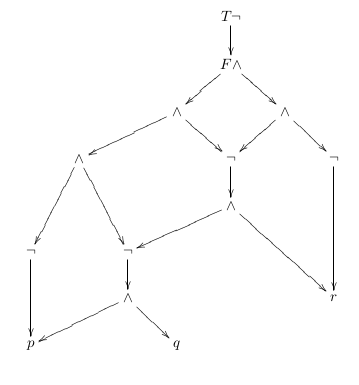
\includegraphics[scale=0.6]{tree.png}}
\put(95,162){F}
\put(157,162){b}
\put(33,134){F}
\put(125,134){d}
\put(185,134){e}
\put(125,107){f}
\put(7,75){F}
\put(65,75){h}
\put(65,50){i}
\put(185,50){j}
\put(7,20){T}
\put(95,20){l}
\end{picture}
\\
In the trees above, we have tried setting node $g$ to $T$ and $F$. We see that we can set no permanent marks and we find no contradictory constraints.\\
\begin{picture}(205,240)
\put(0,0){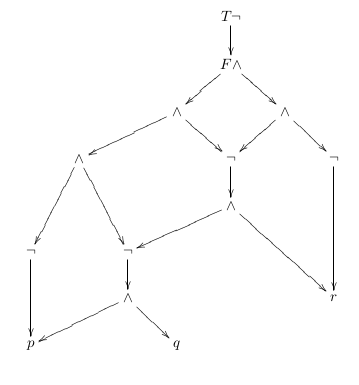
\includegraphics[scale=0.6]{tree.png}}
\put(95,162){F}
\put(157,162){b}
\put(33,134){c}
\put(125,134){d}
\put(185,134){e}
\put(125,107){f}
\put(7,75){g}
\put(65,75){T}
\put(65,50){F}
\put(185,50){j}
\put(7,20){k}
\put(95,20){l}
\end{picture}
\begin{picture}(205,240)
\put(0,0){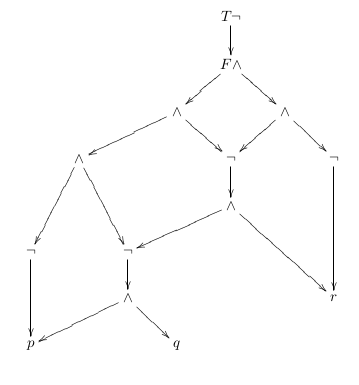
\includegraphics[scale=0.6]{tree.png}}
\put(95,162){F}
\put(157,162){b}
\put(33,134){F}
\put(125,134){T}
\put(185,134){e}
\put(125,107){F}
\put(7,75){F}
\put(65,75){F}
\put(65,50){T}
\put(185,50){j}
\put(7,20){T}
\put(95,20){T}
\end{picture}
\\
In the trees above, we have tried setting node $h$ to $T$ and $F$. We see that we can set no permanent marks and we find no contradictory constraints.\\
\begin{picture}(205,240)
\put(0,0){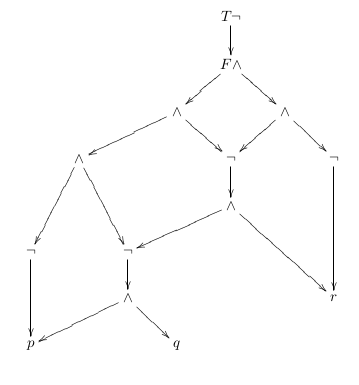
\includegraphics[scale=0.6]{tree.png}}
\put(95,162){F}
\put(157,162){b}
\put(33,134){F}
\put(125,134){T}
\put(185,134){e}
\put(125,107){F}
\put(7,75){F}
\put(65,75){F}
\put(65,50){T}
\put(185,50){j}
\put(7,20){T}
\put(95,20){T}
\end{picture}
\begin{picture}(205,240)
\put(0,0){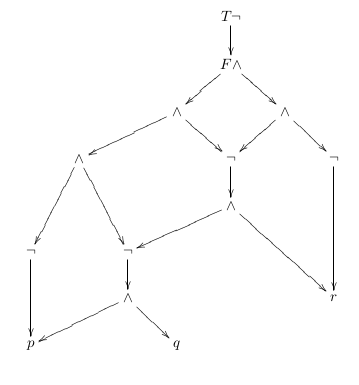
\includegraphics[scale=0.6]{tree.png}}
\put(95,162){F}
\put(157,162){b}
\put(33,134){c}
\put(125,134){d}
\put(185,134){e}
\put(125,107){f}
\put(7,75){g}
\put(65,75){T}
\put(65,50){F}
\put(185,50){j}
\put(7,20){k}
\put(95,20){l}
\end{picture}
\\
In the trees above, we have tried setting node $i$ to $T$ and $F$. We see that we can set no permanent marks and we find no contradictory constraints.\\
\begin{picture}(205,240)
\put(0,0){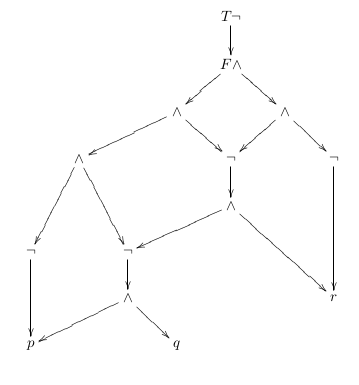
\includegraphics[scale=0.6]{tree.png}}
\put(95,162){F}
\put(157,162){F}
\put(33,134){c}
\put(125,134){d}
\put(185,134){F}
\put(125,107){f}
\put(7,75){g}
\put(65,75){h}
\put(65,50){i}
\put(185,50){T}
\put(7,20){k}
\put(95,20){l}
\end{picture}
\begin{picture}(205,240)
\put(0,0){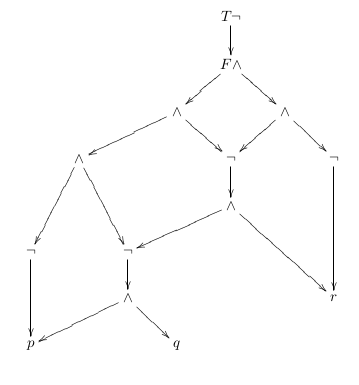
\includegraphics[scale=0.6]{tree.png}}
\put(95,162){F}
\put(157,162){T}
\put(33,134){F}
\put(125,134){T}
\put(185,134){T}
\put(125,107){F}
\put(7,75){g}
\put(65,75){h}
\put(65,50){i}
\put(185,50){F}
\put(7,20){k}
\put(95,20){l}
\end{picture}
\\
In the trees above, we have tried setting node $j$ to $T$ and $F$. We see that we can set no permanent marks and we find no contradictory constraints.\\
\begin{picture}(205,240)
\put(0,0){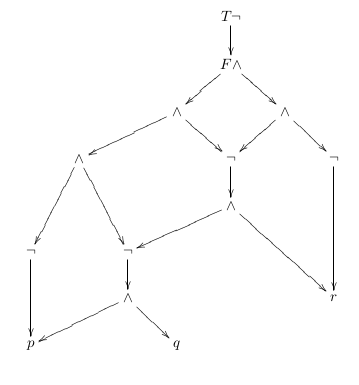
\includegraphics[scale=0.6]{tree.png}}
\put(95,162){F}
\put(157,162){b}
\put(33,134){F}
\put(125,134){d}
\put(185,134){e}
\put(125,107){f}
\put(7,75){F}
\put(65,75){h}
\put(65,50){i}
\put(185,50){j}
\put(7,20){T}
\put(95,20){l}
\end{picture}
\begin{picture}(205,240)
\put(0,0){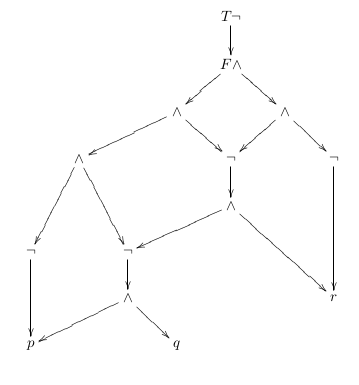
\includegraphics[scale=0.6]{tree.png}}
\put(95,162){F}
\put(157,162){F}
\put(33,134){T}
\put(125,134){F}
\put(185,134){F}
\put(125,107){T}
\put(7,75){T}
\put(65,75){T}
\put(65,50){F}
\put(185,50){T}
\put(7,20){F}
\put(95,20){l}
\end{picture}
\\
In the trees above, we have tried setting node $k$ to $T$ and $F$. We see that we can set no permanent marks and we find no contradictory constraints.\\
\begin{picture}(205,240)
\put(0,0){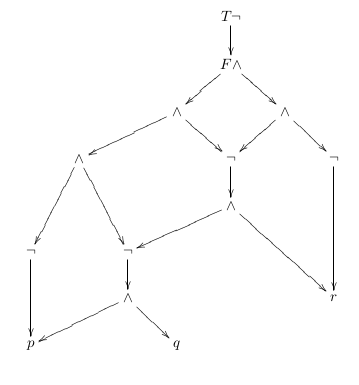
\includegraphics[scale=0.6]{tree.png}}
\put(95,162){F}
\put(157,162){b}
\put(33,134){c}
\put(125,134){d}
\put(185,134){e}
\put(125,107){f}
\put(7,75){g}
\put(65,75){h}
\put(65,50){i}
\put(185,50){j}
\put(7,20){k}
\put(95,20){T}
\end{picture}
\begin{picture}(205,240)
\put(0,0){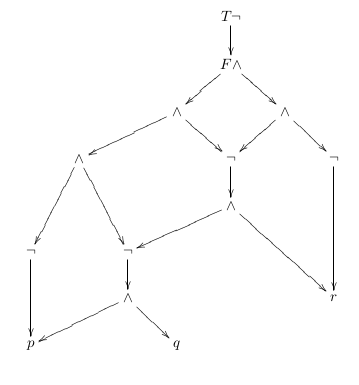
\includegraphics[scale=0.6]{tree.png}}
\put(95,162){F}
\put(157,162){b}
\put(33,134){c}
\put(125,134){d}
\put(185,134){e}
\put(125,107){f}
\put(7,75){g}
\put(65,75){T}
\put(65,50){F}
\put(185,50){j}
\put(7,20){k}
\put(95,20){F}
\end{picture}
\\
In the trees above, we have tried setting node $l$ to $T$ and $F$. We see that we can set no permanent marks and we find no contradictory constraints.\\
This means that the analysis can not decide satisfiability as we want to verify.
\newpage
\subsection*{Completeness exercise}
We want to prove completeness of
$$(p\to q)\to q \vdash (q\to p)\to p$$
We follow the steps described in the assignment text.\\
We start with
$$(p\to q)\to q \models (q\to p)\to p$$
Now we move the premises to the right hand side, so we get
$$\models ((p\to q)\to q)\to((q\to p)\to p)$$
We proceed by creating a truth table
\begin{center}
\begin{tabular}{|c|c||c|c|c|c||c|}
\hline 
$p$ & $q$ & $p\to q$ & $(p\to q)\to q$ & $q\to p$ & $(q\to p)\to p$ & $((p\to q)\to q)\to((q\to p)\to p)$ \\ 
\hline 
T & T & T & T & T & T & T \\ 
\hline 
T & F & F & T & T & T & T \\ 
\hline 
F & T & T & T & F & T & T \\ 
\hline 
F & F & T & F & T & F & T \\ 
\hline 
\end{tabular} 
\end{center}
This means we have the following constructed sequents
\begin{align*}
p,q&\vdash((p\to q)\to q)\to((q\to p)\to p) &:\alpha_1\\
p,\neg q&\vdash((p\to q)\to q)\to((q\to p)\to p) &:\alpha_2\\
\neg p,q&\vdash((p\to q)\to q)\to((q\to p)\to p) &:\alpha_3\\
\neg p,\neg q&\vdash((p\to q)\to q)\to((q\to p)\to p)&:\alpha_4 \\
\end{align*}
As explained in the assignment text, we start by proving $\alpha_1$, meaning we prove
\begin{align*}
p&\vdash \gamma_{\textit{l}}[p] &(a) \\
q&\vdash \gamma_{\textit{l}}[q] &(b)\\
p,q&\vdash \gamma_{\textit{l}}[p\to q]&(c)\\
p,q&\vdash \gamma_{\textit{l}}[(p\to q)\to q]&(d)\\
p,q&\vdash \gamma_{\textit{l}}[q\to p]&(e)\\
p,q&\vdash \gamma_{\textit{l}}[(q\to p)\to p]&(f)\\
p,q&\vdash \gamma_{\textit{l}}[((p\to q)\to q)\to((q\to p)\to p)]&(g)
\end{align*}
In (a), we prove $p\vdash\gamma_{\textit{l}}[p]$ where $\gamma_{\textit{l}}[p]=p$ meaning it is trivially true.\\
In (b), we prove $q\vdash\gamma_{\textit{l}}[q]$ where $\gamma_{\textit{l}}[q]=q$ meaning it is trivially true.\\
In (c), we prove $p,q\vdash\gamma_{\textit{l}}[p\to q]$ where $\gamma_{\textit{l}}[p\to q]=p\to q$. A box proof is provided below
\begin{proofbox}
   \: p 	 \=\mbox{premise}\\
   \: q \= \mbox{premise}
   \[
      \: p		  \=\mbox{assumption}\\
      \: q \=   (2)
   \]
   \: p\to q \= \to I(3-4)
\end{proofbox}
\\
In (d), we prove $p,q\vdash\gamma_{\textit{l}}[(p\to q)\to q]$ where $\gamma_{\textit{l}}[(p\to q)\to q]=(p\to q)\to q$. A box proof is provided below
\begin{proofbox}
   \: p 	 \=\mbox{premise}\\
   \: q \= \mbox{premise}
   \[
     \: p\to q		  \=\mbox{assumption} \\
     \: q \= \to E(1,3)
   \]
   \: (p\to q)\to q \= \to I(3-4)
\end{proofbox}
\\
In (e), we prove $p,q\vdash\gamma_{\textit{l}}[q\to p]$ where $\gamma_{\textit{l}}[q\to p]=q\to p$. This is the exact same proof as in (c), so we reuse this proof with the atoms $p$ and $q$ switched.\\
In (f), we prove $p,q\vdash\gamma_{\textit{l}}[(q\to p)\to p]$ where $\gamma_{\textit{l}}[(q\to p)\to p]=(q\to p)\to p$. This is the exact same proof as in (d), so we reuse this proof with the atoms $p$ and $q$ switched.\\
In (g), we prove $p,q\vdash\gamma_{\textit{l}}[((p\to q)\to q)\to((q\to p)\to p)]$ where $\gamma_{\textit{l}}[((p\to q)\to q)\to((q\to p)\to p)]=((p\to q)\to q)\to((q\to p)\to p)$. A boxproof is provided below
\begin{proofbox}
   \: p 	 \=\mbox{premise}\\
   \: q \= \mbox{premise}\\
   \: (p\to q)\to q \= \mbox{proved in (d)}\\
   \: (q\to p)\to p \= \mbox{proved in (f)}
   \[
     \: (p\to q)\to q		  \=\mbox{assumption} \\
     \: (q\to p)\to p \= (4)
   \]
   \: ((p\to q)\to q)\to ((q\to p)\to p) \= \to I(5-6)
\end{proofbox}
We now prove $\alpha_2$ in the same manner.
\begin{align*}
p&\vdash \gamma_{\textit{l}}[p] &(a) \\
\neg q&\vdash \gamma_{\textit{l}}[q] &(b)\\
p,\neg q&\vdash \gamma_{\textit{l}}[p\to q]&(c)\\
p,\neg q&\vdash \gamma_{\textit{l}}[(p\to q)\to q]&(d)\\
p,\neg q&\vdash \gamma_{\textit{l}}[q\to p]&(e)\\
p,\neg q&\vdash \gamma_{\textit{l}}[(q\to p)\to p]&(f)\\
p,\neg q&\vdash \gamma_{\textit{l}}[((p\to q)\to q)\to((q\to p)\to p)]&(g)
\end{align*}
In (a), we prove $p\vdash\gamma_{\textit{l}}[p]$ where $\gamma_{\textit{l}}[p]=p$ meaning it is trivially true.\\
In (b), we prove $\neg q\vdash\gamma_{\textit{l}}[q]$ where $\gamma_{\textit{l}}[q]=\neg q$ meaning it is trivially true.\\
In (c), we prove $p,\neg q\vdash\gamma_{\textit{l}}[p\to q]$ where $\gamma_{\textit{l}}[p\to q]=\neg(p\to q)$. A box proof is provided below
\begin{proofbox}
   \: p 	 \=\mbox{premise}\\
   \: \neg q \= \mbox{premise}
   \[
      \: (p\to q)		  \=\mbox{assumption}\\
      \: q \= \to E(1,3) \\
      \: \bot \= \neg E(4,2) 
   \]
   \: \neg(p\to q) \= \neg I(3-5)
\end{proofbox}
\\
In (d), we prove $p,\neg q\vdash\gamma_{\textit{l}}[(p\to q)\to q]$ where $\gamma_{\textit{l}}[(p\to q)\to q]=(p\to q)\to q$. A box proof is provided below
\begin{proofbox}
   \: p 	 \=\mbox{premise}\\
   \: \neg q \= \mbox{premise}
   \[
     \: p\to q		  \=\mbox{assumption} \\
     \: q \= \to E(1,3)
   \]
   \: (p\to q)\to q \= \to I(3-4)
\end{proofbox}
\\
In (e), we prove $p,\neg q\vdash\gamma_{\textit{l}}[q\to p]$ where $\gamma_{\textit{l}}[q\to p]=q\to p$. A box proof is provided below
\begin{proofbox}
   \: p 	 \=\mbox{premise}\\
   \: \neg q \= \mbox{premise}
   \[
     \: q		  \=\mbox{assumption} \\
     \: \bot \= \neg E(3,2)
     \: p
   \]
   \: q\to p \= \to I(3-5)
\end{proofbox}
\\
In (f), we prove $p,q\vdash\gamma_{\textit{l}}[(q\to p)\to p]$ where $\gamma_{\textit{l}}[(q\to p)\to p]=(q\to p)\to p$. A box proof is provided below
\begin{proofbox}
   \: p 	 \=\mbox{premise}\\
   \: \neg q \= \mbox{premise}
   \[
     \: (q\to p)		  \=\mbox{assumption} \\
     \: p \= (1)
   \]
   \: (q\to p)\to p \= \to I(3-4)
\end{proofbox}
\\
In (g), we prove $p,\neg q\vdash\gamma_{\textit{l}}[((p\to q)\to q)\to((q\to p)\to p)]$ where $\gamma_{\textit{l}}[((p\to q)\to q)\to((q\to p)\to p)]=((p\to q)\to q)\to((q\to p)\to p)$. A boxproof is provided below
\begin{proofbox}
   \: p 	 \=\mbox{premise}\\
   \: \neg q \= \mbox{premise}\\
   \: (p\to q)\to q \= \mbox{proved in (d)} \\
   \: (q\to p)\to p \= \mbox{proved in (f)} \\
   \[
     \: (p\to q)\to q		  \=\mbox{assumption} \\
     \: (q\to p)\to p \= (4)
   \]
   \: ((p\to q)\to q)\to((q\to p)\to p) \= \to I(5-6)
\end{proofbox}
We now prove $\alpha_3$ in the same manner.
\begin{align*}
\neg p&\vdash \gamma_{\textit{l}}[p] &(a) \\
q&\vdash \gamma_{\textit{l}}[q] &(b)\\
\neg p,q&\vdash \gamma_{\textit{l}}[p\to q]&(c)\\
\neg p,q&\vdash \gamma_{\textit{l}}[(p\to q)\to q]&(d)\\
\neg p,q&\vdash \gamma_{\textit{l}}[q\to p]&(e)\\
\neg p,q&\vdash \gamma_{\textit{l}}[(q\to p)\to p]&(f)\\
\neg p,q&\vdash \gamma_{\textit{l}}[((p\to q)\to q)\to((q\to p)\to p)]&(g)
\end{align*}
In (a), we prove $\neg p\vdash\gamma_{\textit{l}}[p]$ where $\gamma_{\textit{l}}[p]=\neg p$ meaning it is trivially true.\\
In (b), we prove $q\vdash\gamma_{\textit{l}}[q]$ where $\gamma_{\textit{l}}[q]=q$ meaning it is trivially true.\\
In (c), we prove $\neg p,q\vdash\gamma_{\textit{l}}[p\to q]$ where $\gamma_{\textit{l}}[p\to q]=p\to q$. A box proof is provided below
\begin{proofbox}
   \: \neg p 	 \=\mbox{premise}\\
   \: q \= \mbox{premise}
   \[
      \: p		  \=\mbox{assumption}\\
      \: \bot \= \neg E(3,1) \\
      \: q \= \bot E(4)
   \]
   \: p\to q \= \to I(3-5)
\end{proofbox}
\\
In (d), we prove $\neg p,q\vdash\gamma_{\textit{l}}[(p\to q)\to q]$ where $\gamma_{\textit{l}}[(p\to q)\to q]=(p\to q)\to q$. A box proof is provided below
\begin{proofbox}
   \: \neg p 	 \=\mbox{premise}\\
   \: q \= \mbox{premise}
   \[
     \: p\to q		  \=\mbox{assumption} \\
     \: q \= (2)
   \]
   \: (p\to q)\to q \= \to I(3-4)
\end{proofbox}
\\
In (e), we prove $\neg p,q\vdash\gamma_{\textit{l}}[q\to p]$ where $\gamma_{\textit{l}}[q\to p]=\neg(q\to p)$. A box proof is provided below
\begin{proofbox}
   \: \neg p 	 \=\mbox{premise}\\
   \: q \= \mbox{premise}
   \[
     \: q\to p		  \=\mbox{assumption} \\
     \: p \= \to E(2,3) \\
     \: \bot \= \neg I(4,1)
   \]
   \:  \neg(q\to p) \= \neg E(3-5)
\end{proofbox}
\\
In (f), we prove $\neg p,q\vdash\gamma_{\textit{l}}[(q\to p)\to p]$ where $\gamma_{\textit{l}}[(q\to p)\to p]=(q\to p)\to p$. A box proof is provided below
\begin{proofbox}
   \: \neg p 	 \=\mbox{premise}\\
   \: q \= \mbox{premise}
   \[
     \: q\to p		  \=\mbox{assumption} \\
     \: p \= \to E(2,3)
   \]
   \:  (q\to p)\to p \= \to I(3-4)
\end{proofbox}
\\
In (g), we prove $\neg p,q\vdash\gamma_{\textit{l}}[((p\to q)\to q)\to((q\to p)\to p)]$ where $\gamma_{\textit{l}}[((p\to q)\to q)\to((q\to p)\to p)]=((p\to q)\to q)\to((q\to p)\to p)$. A boxproof is provided below
\begin{proofbox}
   \: \neg p 	 \=\mbox{premise}\\
   \: q \= \mbox{premise}\\
   \: (p\to q)\to q \= \mbox{proved in (d)} \\
   \: (q\to p)\to p \= \mbox{proved in (f)}
   \[
     \: (p\to q)\to q	  \=\mbox{assumption} \\
     \: (q\to p)\to p\= (4)
   \]
   \: ((p\to q)\to q)\to((q\to p)\to p) \= \to I(5-6)
\end{proofbox}
We now prove $\alpha_4$ in the same manner.
\begin{align*}
\neg p&\vdash \gamma_{\textit{l}}[p] &(a) \\
\neg q&\vdash \gamma_{\textit{l}}[q] &(b)\\
\neg p,\neg q&\vdash \gamma_{\textit{l}}[p\to q]&(c)\\
\neg p,\neg q&\vdash \gamma_{\textit{l}}[(p\to q)\to q]&(d)\\
\neg p,\neg q&\vdash \gamma_{\textit{l}}[q\to p]&(e)\\
\neg p,\neg q&\vdash \gamma_{\textit{l}}[(q\to p)\to p]&(f)\\
\neg p,\neg q&\vdash \gamma_{\textit{l}}[((p\to q)\to q)\to((q\to p)\to p)]&(g)
\end{align*}
In (a), we prove $\neg p\vdash\gamma_{\textit{l}}[p]$ where $\gamma_{\textit{l}}[p]=\neg p$ meaning it is trivially true.\\
In (b), we prove $\neg q\vdash\gamma_{\textit{l}}[q]$ where $\gamma_{\textit{l}}[q]=\neg q$ meaning it is trivially true.\\
In (c), we prove $\neg p,\neg q\vdash\gamma_{\textit{l}}[p\to q]$ where $\gamma_{\textit{l}}[p\to q]=p\to q$. A box proof is provided below
\begin{proofbox}
   \: \neg p 	 \=\mbox{premise}\\
   \: \neg q \= \mbox{premise}
   \[
      \: p		  \=\mbox{assumption}\\
      \: \bot \= \to E(3,1) \\
      \: q \= \bot E(4)
   \]
   \: p\to q \= \to I(3-5)
\end{proofbox}
\\
In (d), we prove $\neg p,\neg q\vdash\gamma_{\textit{l}}[(p\to q)\to q]$ where $\gamma_{\textit{l}}[(p\to q)\to q]=\neg((p\to q)\to q)$. A box proof is provided below
\begin{proofbox}
   \: \neg p 	 \=\mbox{premise}\\
   \: \neg q \= \mbox{premise} \\
   \: p\to q	 \= \mbox{proved in (c)}
   \[
     \: (p\to q)\to q		  \=\mbox{assumption} \\
     \: q \= \to E(3,4) \\
     \: \bot \= \neg E(5,2)
   \]
   \: \neg((p\to q)\to q) \= \neg I(4-6)
\end{proofbox}
\\
In (e), we prove $\neg p,\neg q\vdash\gamma_{\textit{l}}[q\to p]$ where $\gamma_{\textit{l}}[q\to p]=q\to p$. A box proof is provided below
\begin{proofbox}
   \: \neg p 	 \=\mbox{premise}\\
   \: \neg q \= \mbox{premise}
   \[
     \: q		  \=\mbox{assumption} \\
     \: \bot \= \neg E(3,2) \\
     \: p \= \bot E(4)
   \]
   \:  q\to p \= \to I(3-5)
\end{proofbox}
\\
In (f), we prove $\neg p,\neg q\vdash\gamma_{\textit{l}}[(q\to p)\to p]$ where $\gamma_{\textit{l}}[(q\to p)\to p]=\neg((q\to p)\to p)$. A box proof is provided below
\begin{proofbox}
   \: \neg p 	 \=\mbox{premise}\\
   \: \neg q \= \mbox{premise} \\
   \: (q\to p) \= \mbox{proved in (e)}
   \[
     \: (q\to p)\to p		  \=\mbox{assumption} \\
     \: p \= \to E(3,4) \\
     \: \bot \= \neg E(5,1)
   \]
   \:  \neg((q\to p)\to p) \= \neg I(4-6)
\end{proofbox}
\newpage
In (g), we prove $\neg p,\neg q\vdash\gamma_{\textit{l}}[((p\to q)\to q)\to((q\to p)\to p)]$ where $\gamma_{\textit{l}}[((p\to q)\to q)\to((q\to p)\to p)]=((p\to q)\to q)\to((q\to p)\to p)$. A boxproof is provided below
\begin{proofbox}
   \: p 	 \=\mbox{premise}\\
   \: q \= \mbox{premise}\\
   \: \neg((p\to q)\to q) \= \mbox{proved in (d)} \\
   \: \neg((q\to p)\to p) \= \mbox{proved in (f)}
   \[
     \: (p\to q)\to q	  \=\mbox{assumption} \\
     \: \bot \= \neg E(5,3) \\
     \: (q\to p)\to p \= \bot E(6)
   \]
   \: ((p\to q)\to q)\to((q\to p)\to p) \= \to I(5-7)
\end{proofbox}
These proofs $\alpha_1,\alpha_2,\alpha_3$ and $\alpha_4$ together can be used to prove that 
$$\vdash ((p\to q)\to q)\to((q\to p)\to p)$$
as all combination of truth values are used.\\
We extend this to to the proof
$$(p\to q)\to q\vdash (q\to p)\to p$$
As so we have proved completeness of the formula.

\end{document}